\documentclass[a4paper]{article}

\usepackage[a4paper,  margin=0.5in]{geometry}
% \usepackage[left=2.5cm,top=3cm,right=2.5cm,bottom=3cm,bindingoffset=0.5cm]{geometry}

\usepackage{graphicx}
\usepackage{float}
\usepackage{hyperref}
\usepackage{multicol}


\usepackage[utf8]{inputenc}
\begin{document}

% \begin{titlepage}
\title{SNR classes project - birds species recognition using deep neural networks
- first stage report}

\author{Michał Sypetkowski, Marcin Lew}
\maketitle
% \end{titlepage}





% \tableofcontents
% \addcontentsline{toc}{section}{Contents}
% \newpage


\begin{multicols}{2}

\section{General information}
Git repository \url{https://github.com/msypetkowski/SNR-proj.git}.
We use the following tools:
\begin{itemize}
    \item \textbf{Python}\cite{Python}
    \item \textbf{OpenCV}\cite{OpenCV}
    \item \textbf{NumPy}\cite{NumPy}
    \item \textbf{TensorFlow}\cite{TensorFlow}
\end{itemize}
We also use Tensorboard for model and training progress visualization.
The project is tested to run in Linux environment.

\section{Multilayer Perceptron}

\subsection{Data}
Dataset consists of 50 subsets -- types of bird species.
Each subset is a set of 60 different pictures.
Altogether it gives us a data set of 3000 pictures.

We divided this dataset, so that there are 300 examples in test set and
2700 examples in training set.
Number of examples per each class is equal in both training and test set
(54 examples per class in training set and 6 in test set).
Additionally, training set is augmented during training (see section \ref{augmentation}).


\subsection{Data augmentation}
\label{augmentation}
Every training image is randomly rotated, flipped or cropped.
Augmentation is done online, so the number of training examples is
roughly infinite.
We skip the distributions of the transformations in this document.
Instead we attach an example visualization.
Raw -- unaugmented example (center crop) is shown in figure \ref{fig:aug1}.
Corresponding augmented examples are shown in figure \ref{fig:aug2}.

% TODO: was there a special name for unaugmened examples ?

\begin{figure}[H]
    \caption[]{Not augmented example}
    \centering
    \includegraphics[page=2,width=0.1\textwidth]{aug1.png}
    \label{fig:aug1}
\end{figure}

\begin{figure}[H]
    \caption[]{Augmented examples corresponding to raw example in figure \ref{fig:aug1}}
    \centering
    \includegraphics[page=2,width=0.5\textwidth]{aug2.png}
    \label{fig:aug2}
\end{figure}

\subsection{HOG features}
To get HOG features, we first resize an image to 128x64x3.
Then we calculate the features using OpenCV library:
\begin{verbatim}
    hog = cv2.HOGDescriptor()
    fd = hog.compute(img).flatten()
\end{verbatim}

Image is first divided into 8x8 cells (in result, we get 16 * 8 cells).
We use gradient orientation bins of size 9.
Then the algorithm takes 16x16 blocks (4 cells) --
there are 7 * 15 such blocks.
Histograms of each of 4 cells in block are concatenated and L2 normalized.
In the end, all blocks histograms are concatenated giving
final feature vecor of length (7 * 15) * 36 = 3780.
We directly feed such vectors into our network.

\subsection{Model architecture}
We selected the architecture by experimenting.
Our network has 3 hidden dense layers of sizes 256, 128 and 64.
Since we have small dataset, larger models tended to overfit
(despite of data augmentation).
Each of these layers have corresponding batch normalization\cite{Batchnorm} layer.
After the last layer there is a softmax function.
We use cross entropy as a loss function.
We tested 2 models with different activation functions -- relu and sigmoid.

Visualization of the model (with relu activation) is shown in figure \ref{fig:arch}.

% TODO: draw different - more simple schema instead of tensorboard printscreen
\begin{figure}[H]
    \caption[]{Visualization of multilayer perceptron architecture (relu activation variant)}
    \centering
    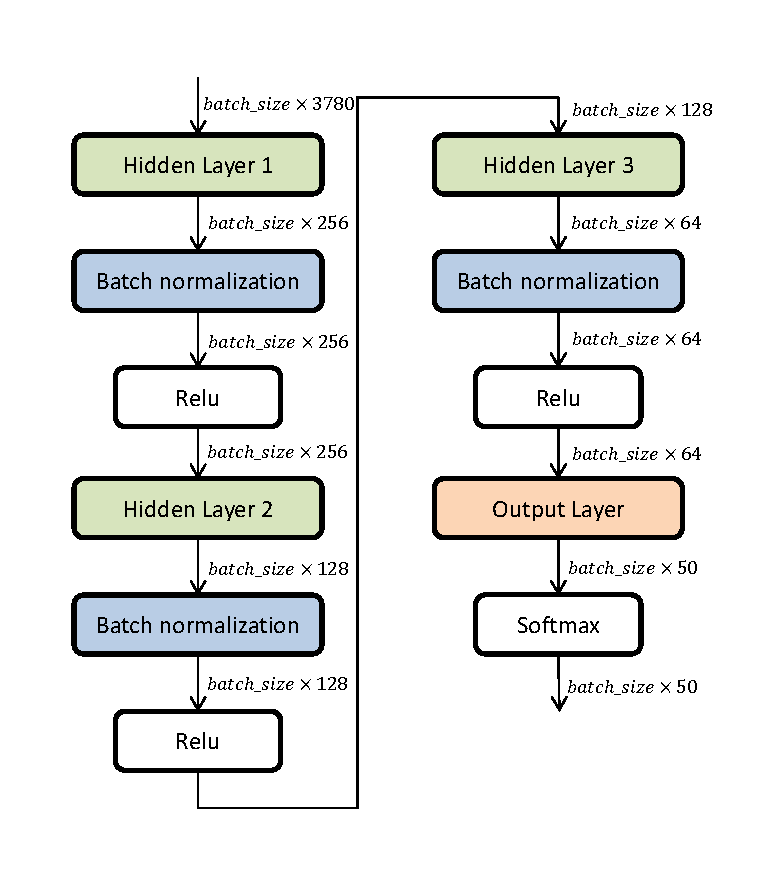
\includegraphics[page=1,width=0.5\textwidth]{architecture.pdf}
    \label{fig:arch}
\end{figure}


\subsection{Training and results}
Training and validation curves are shown in figures \ref{fig:training_accuracy} and \ref{fig:training_loss}.
For each model, they diverge from the begining because of small dataset (one epoch is around 20 iterations).
Because of batch normalization\cite{Batchnorm} layers, validation accuracy increases along with training accuracy (but slower).
Full results on testset for the model using relu are shown in figure \ref{fig:eval}.

Final accuracy of relu model is around 24\%.
Sigmoid model achieves slightly lower accuracy (around 21\%).
Nowadays, it is a common knowledge that using relu as activation function
usually gives faster and better results i. a. for classification tasks;
hence the result is not surprising.





\section{Convolutional neural networks}

\subsection{"Ground truth" model}

We trained for 1500 iterations 8-th layer of VGG16\cite{VGG16}
pretrained on ImageNet\cite{ImageNet} dataset.
Then we finetuned it for 1000 iterations achieving final accuracy of 67\%.
Training and validation curves are shown in figure \ref{fig:trainingVGG_accuracy}. % and \ref{fig:trainingVGG_loss}.
Full results on testset shown in figure \ref{fig:evalVGG}.
The ckpt file is downloaded from \url{http://download.tensorflow.org/models/vgg_16_2016_08_28.tar.gz}.

\subsection{Next stage plans}

We are planning to experiment with convolutional neural network architectures
without using pretrained models.
i.a. with:
\begin{itemize}
    \item convolutional layers count
    \item loss function
    \item activation function
    \item using SVM (with various exponential kernels) after the last network layer

\end{itemize}




\end{multicols}

% TODO: hide the fact that this is tensorboard printscreen or do other - external visualization
\begin{figure}[h]
    \caption[]{Accuracy graph for a multi-layer perceptron.}
    \centering
    \includegraphics[page=2,width=0.9\textwidth]{training_accuracy.png}
    \label{fig:training_accuracy}
\end{figure}

\begin{figure}[h]
    \caption[]{Loss graph for a multi-layer perceptron.}
    \centering
    \includegraphics[page=2,width=0.9\textwidth]{training_loss.png}
    \label{fig:training_loss}
\end{figure}

\begin{figure}[H]
    \caption[]{Training and validation accuracy curves for the VGG16 pretrained model (orange line is for validation)}
    \centering
    \includegraphics[page=2,width=1.0\textwidth]{vggTraining_accuracy.png}
    \label{fig:trainingVGG_accuracy}
\end{figure}

% \begin{figure}[h]
%     \caption[]{Loss graph for the VGG16 pretrained model.}
%     \centering
%     \includegraphics[page=2,width=1.0\textwidth]{vggTraining_loss.png}
%     \label{fig:trainingVGG_loss}
% \end{figure}


\begin{figure}[h]
    \caption[]{Results on testset of VGG16 finetuned model (blue - correct answers).}
    \centering
    \includegraphics[page=2,width=1.0\textwidth]{evalVGG.png}
    \label{fig:evalVGG}
\end{figure}

\begin{figure}[h]
    \caption[]{Results on testset of small model that uses HOG features (blue - correct answers)}
    \centering
    \includegraphics[page=2,width=1.0\textwidth]{eval.png}
    \label{fig:eval}
\end{figure}


% Since we have small dataset, we are not sure if a very deep architecture
% will be efficient in our case.
% Eventually, we will consider architectures designed
% for more shallow models (e.g. VGG \footnote{\url{https://arxiv.org/abs/1409.1556}}).
% We are planning to use {ResNet}\footnote{\url{https://arxiv.org/abs/1512.03385}}
% as a baseline model.

\clearpage
\begin{thebibliography}{99}
\addcontentsline{toc}{section}{References}

\bibitem{TensorFlow} Google Brain team. \url{https://www.tensorflow.org/}, (09.05.2018).

\bibitem{NumPy} NumPy developers. \url{http://www.numpy.org/}, (09.05.2018).

\bibitem{OpenCV} OpenCV team. \url{https://opencv.org/}, (09.05.2018).

\bibitem{Python} Python Software Foundation. \url{https://www.python.org/}, (09.05.2018).

\bibitem{ImageNet}Russakovsky O., Deng J., Su H., Krause J., Satheesh S., Ma S., Huang Z., Karpathy A., Khosla A., Bernstein M., Berg A. C., Fei-Fei L.: \textit{ImageNet Large Scale Visual Recognition Challenge}, 2014. 
\url{https://arxiv.org/abs/1409.0575}, (09.05.2018).

\bibitem{VGG16}Simonyan K., Zisserman A.: \textit{Very Deep Convolutional Networks for Large-Scale Image Recognition}, 2014. \url{https://arxiv.org/abs/1409.1556}, (09.05.2018).

\bibitem{Batchnorm} Sergey Ioffe and Christian Szegedy: \textit{Batch Normalization: Accelerating Deep Network Training by Reducing Internal Covariate Shift}, 2015. \url{http://arxiv.org/abs/1502.03167}, (10.05.2018).

\end{thebibliography}

\end{document}
